% Chapter Template

\chapter{Laminated Composite Material Optimization by New Genetic Algorithm Model} % Main chapter title

\label{Chapter4} % Change X to a consecutive number; for referencing this chapter elsewhere, use \ref{ChapterX}


\section{Case1: Maximum Strength Optimization}
\begin{table*}[!ht]
\normalsize
\caption{Properties of T300/5308 carbon/epoxy composite}
\label{tab:T300/5308}
\centering
\begin{tabularx}{1.0\textwidth}{p{0.5\textwidth}p{0.1\textwidth}p{0.1\textwidth}c}
	\toprule
	\textbf{Property}								   & \textbf{Symbol}				  & \textbf{Unit}  & \textbf{ Graphite/Epoxy}     \\
	\midrule
	Longitudinal elastic modulus			   & $E_1$				  & GPa   &  181                 \\
	Traverse elastic modulus				   & $E_2$				  & GPa   &  10.3                \\
	Major Poisson's ratio					   & $v_{12}$			  &       &  0.28                \\
	Shear modulus							   & $G_{12}$			  & GPa   &  7.17                \\
	Ultimate longitudinal tensile strength     & $(\sigma_1^T)_{ult}$ & MP    &  1500                 \\
	Ultimate longitudinal compressive strength & $(\sigma_1^C)_{ult}$ & MP    &  1500                 \\
	Ultimate transverse tensile strength       & $(\sigma_2^T)_{ult}$ & MPa   &  40                   \\
	Ultimate transverse compressive strength   & $(\sigma_2^C)_{ult}$ & MPa   &  246                   \\
	Ultimate in-plane shear strength           & $(\tau_{12})_{ult}$  & MPa   &  68                    \\
	\bottomrule
\end{tabularx}
\end{table*}


\subsection{Methodology}
\subsection{Result and Discussion}

\section{Case2: Minimum Thickness Optimization}

\subsection{Methodology}


\begin{figure}[!htb]
	\centering
		\begin{subfigure}[b]{0.8\linewidth}
			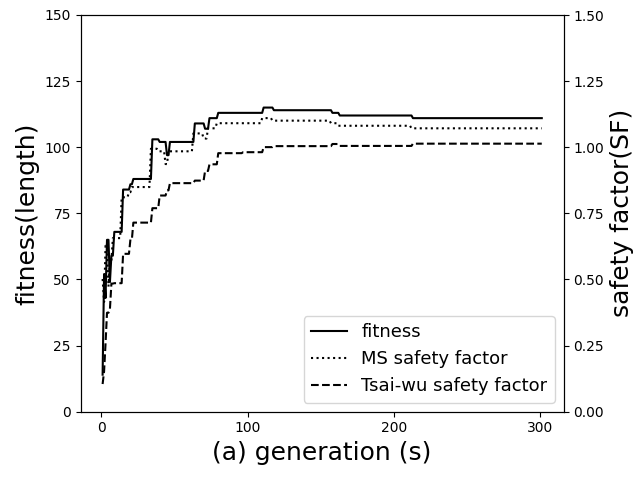
\includegraphics[width=\linewidth]{Figures/chapter4_second_two_distinct_angle_fitness_and_sr.png}
		\end{subfigure}

		\begin{subfigure}[b]{0.8\linewidth}
			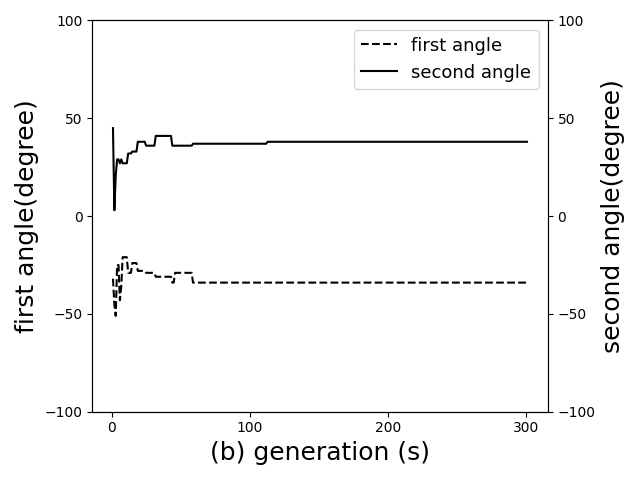
\includegraphics[width=\linewidth]{Figures/chapter4_second_two_distinct_angle_angle_change.png}
		\end{subfigure}

		\begin{subfigure}[b]{0.8\linewidth}
			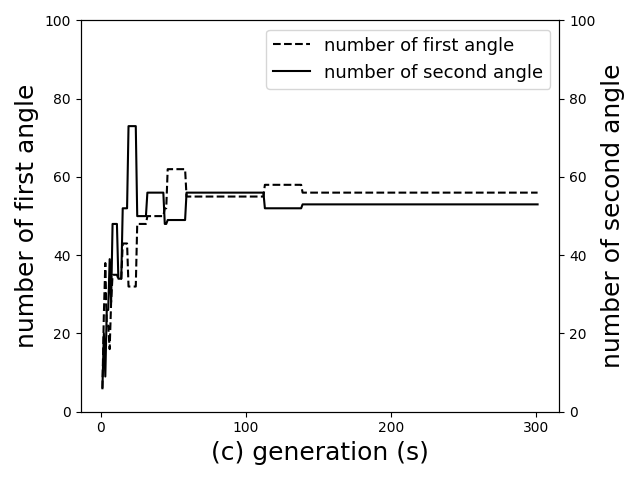
\includegraphics[width=\linewidth]{Figures/chapter4_second_two_distinct_angler_number_change.png}
		\end{subfigure}
	\caption{Two distinct angles}
	\label{fig:two_angles}
\end{figure}

\begin{table*}
	\normalsize
\caption{The optimum lay-ups using two distinct fiber angles under various biaxial loading cases}
\label{tab:two_distinct_angle}
\centering
\resizebox{13cm}{!}{
\begin{tabular}{clccc}
	\toprule
	\textbf{Loading} $N_{x}/N_{y}/N_{xy}$ \textbf{(MPa m)}   &
	\makecell{\textbf{Optimum lay-up } \\ \textbf{sequences}  }                        &
	\textbf{Laminate thickness} &  \makecell{\textbf{Safety factor } \\
	\textbf{for Tsai-wu}}  &
	\makecell{\textbf{Safety factor } \\ \textbf{for  maximum stress}}
	 \\
	\midrule
	10/5/0                                         &  $[33_{29}/\text{-}39_{25}/\bar{\text{-}39}]_s$            &     109               &  1.0074      &  1.0246  \\
	20/5/0                                         &  $[33_{22}/\text{-}31_{24}]_s$                             &     92               &  1.0055       &  1.2065    \\
	40/5/0                                         &  $[29_{18}/\text{-}21_{23}/\bar{\text{-}21}]_s$            &     83               &  1.0034       &  1.7350   \\
	80/5/0                                         &  $[\text{-}20_{27}/21_{25}/\bar{25}]_s$                    &     105               &  1.0029      &  1.2063    \\
	120/5/0                                         &  $[\text{-}18_{34}/17_{36}]_s$                            &     140               &  1.0000      &  1.0898    \\
	\bottomrule
\end{tabular}
}
\end{table*}







\begin{figure}[!htb]
	\centering
		\begin{subfigure}[b]{0.8\linewidth}
			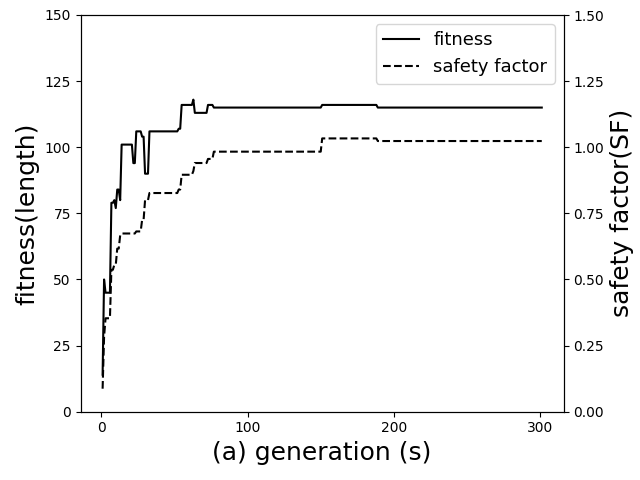
\includegraphics[width=\linewidth]{Figures/chapter4_second_three_distinct_angle_fitness_and_sr.png}
		\end{subfigure}

		\begin{subfigure}[b]{0.8\linewidth}
			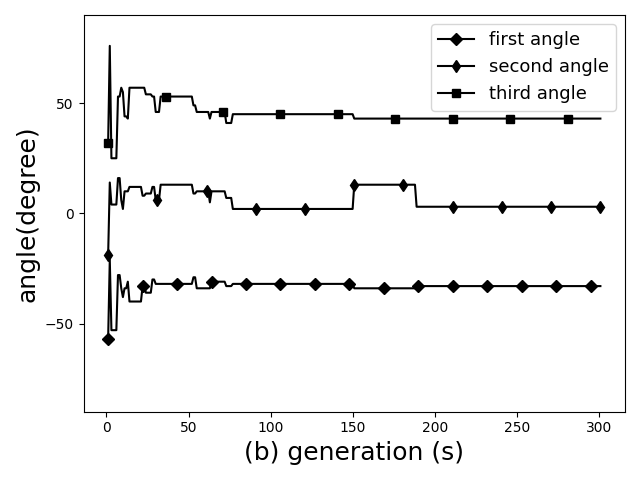
\includegraphics[width=\linewidth]{Figures/chapter4_second_three_distinct_angle_angle_change.png}
		\end{subfigure}

		\begin{subfigure}[b]{0.8\linewidth}
			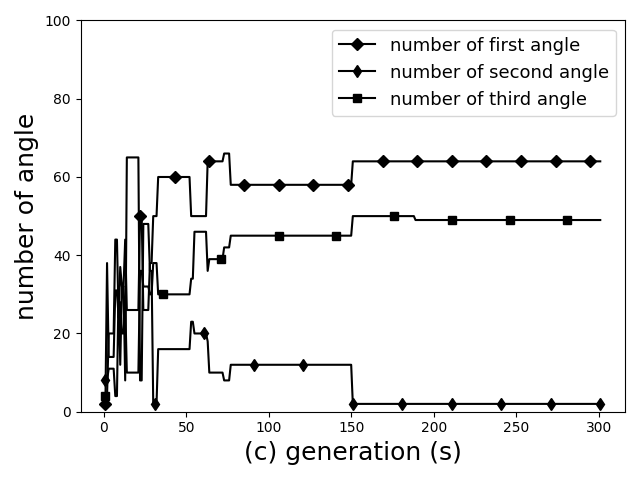
\includegraphics[width=\linewidth]{Figures/chapter4_second_three_distinct_angler_number_of_angle.png}
		\end{subfigure}
	\caption{three distinct angles}
	\label{fig:three_angles}
\end{figure}
\begin{table*}
\normalsize
\caption{The optimum lay-ups using three distinct fiber angles under various biaxial loading cases}
\label{T300/5308 material properties}
\centering
\resizebox{13cm}{!}{
\begin{tabular}{clccc}
	\toprule
	\textbf{Loading} $N_{x}/N_{y}/N_{xy}$ \textbf{(MPa m)}   &
	\makecell{\textbf{Optimum lay-up } \\ \textbf{sequences}  }                        &
	\textbf{Laminate thickness} &  \makecell{\textbf{Safety factor } \\
	\textbf{for Tsai-wu}}  &
	\makecell{\textbf{Safety factor } \\ \textbf{for  maximum stress}}
	 \\
	\midrule
	10/5/0                       &  $[37_{27}/\text{-}38_{27}/\text{-}5]_s$            &     110      &  1.0023 & 1.0216\\
	20/5/0                       &  $[34_{24}/\text{-}32_{14}/\text{-}28_{11}]_s$      &     98       &  1.0237 & 1.2089 \\
	40/5/0                       &  $[21_{28}/\text{-}32_{19}/2_3]_s$                  &     100      &  1.0617 & 1.7076\\
	80/5/0                       &  $[\text{-}19_{24}/20_{27}/\text{-}{17}_{16}/\bar{\text{-}17}]_s$  &  109      &  1.0056 & 1.2093 \\
	120/5/0                      &  $[\text{-}19_{33}/12_{13}/16_{28}]_s$              &     148      &  1.0105 &  1.1014\\
	\bottomrule
\end{tabular}
}
\end{table*}


\begin{table*}
	\normalsize
\caption{Comparison with the results of DSA}
\label{tab:comparision}
\centering
\resizebox{13cm}{!}{
\begin{tabular}{c|cccc|lccc}
	\toprule
	\textbf{Loading}	    & \multicolumn {4}{c}{\textbf{Akbulut and Sonmez's\cite{akbulut2008optimum} Study}}   & \multicolumn {4}{c}{\textbf{Present Study}}\\
	\midrule
	 $N_{x}/N_{y}/N_{xy}$   & Optimum lay-up			        & laminate  & TW & MS   & Optimum lay-up & laminate  & TW & MS \\
	  (MPa m)	            & sequences					        & thickness &    &      & sequences	     & thickness &    &    \\
	\midrule
	  10/5/0                 &  $[37_{27}/\text{-}37_{27}]_s$     &  108      &  1.0068  &  1.0277 & $[33_{29}/\text{-}39_{25}/\bar{\text{-}39}]_s$     &     109      &  1.0074      &  1.0246  \\
	  20/5/0                 &  $[31_{23}/\text{-}31_{23}]_s$     &  92       &  1.0208  &  1.1985 & $[33_{22}/\text{-}31_{24}]_s$                      &     92      &  1.0055       &  1.2065    \\
	  40/5/0                 &  $[26_{20}/\text{-}26_{20}]_s$     &  80       &  1.0190  &  1.5381 & $[29_{18}/\text{-}21_{23}/\bar{\text{-}21}]_s$     &     83      &  1.0034       &  1.7350   \\
	  80/5/0                 &  $[21_{25}/\text{-}19_{28}]_s$     &  106      &  1.0113  &  1.2213 & $[\text{-}20_{27}/21_{25}/\bar{25}]_s$             &     105      &  1.0029      &  1.2063    \\
	  120/5/0                &  $[17_{35}/\text{-}17_{35}]_s$     &  140      &  1.0030  &  1.0950 & $[\text{-}18_{34}/17_{36}]_s$                     &     140      &  1.0000      &  1.0898     \\
	\bottomrule
\end{tabular}
}
\end{table*}

\subsection{Result and Discussion}

\section{Summary}

